\subsection{A demonstrative example}\label{sec:example}
To illustrate the different


\begin{figure}
\centering
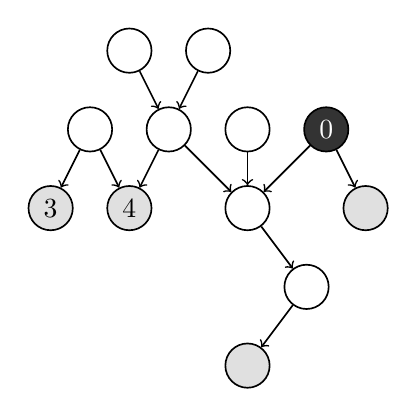
\begin{tikzpicture}[semithick]
\tikzset{ every node/.style={circle, draw, fill=white, minimum size=16pt, inner sep=1pt}}
\tikzstyle{note}=[draw=white,fill=white,font=\small,circle,inner sep=0pt]
\tikzstyle{evidence}=[fill=gray!24]
\tikzstyle{query}=[fill=black!80, text=white]
\tikzstyle{ed}=[draw=black,line width=.8pt, postaction={decorate}, decoration={markings,mark=at position 1.0 with {\arrow[draw=black,line width=.8pt]{>}}}]
%\begin{scope}
% vertices
\node (a) at (0,1) {};
\node (b) at (1,1) {};
\node (c) at (2,1) {};
\node[query] (d) at (3,1) {0};
\node[evidence] (e) at (-.5,0) {3};
\node[evidence] (f) at (0.5,0) {4};
\node (g) at (2,0) {};
\node[evidence] (h) at (3.5,0) {};
\node (m) at (2.75,-1) {};
\node[evidence] (n) at (2,-2) {};
\node[] (o) at (1.5,2) {};
\node[] (p) at (.5,2) {};
%\node[note] (label) at (1,-1) {(a)};
\draw[->] (a) -- (e);
\draw[->] (a) -- (f);
\draw[->] (b) -- (f);
\draw[->] (b) -- (g);
\draw[->] (c) -- (g);
\draw[->] (d) -- (g);
\draw[->] (d) -- (h);
\draw[->] (g) -- (m);
\draw[->] (m) -- (n);
\draw[->] (o) -- (b);
\draw[->] (p) -- (b);
%\end{scope}
%\begin{scope}[xshift=5cm]
%\end{scope}
\end{tikzpicture}
\caption{A polytree-shaped credal network}
\label{fig:polytree}
\end{figure}






